\chapter{Automatizált Internet mérő rendszer}
%(13-15 oldal): 

Jelen fejezet mutatja be az elkészült automatizált mérési rendszert, annak felépítését és működési elvét.

\section{Mérési elrendezés}
%(5 oldal): traceroute, iperf, mérési forgatókönyvek, PlanetLab

A felhőben vagy kliensen futó szoftver óránként felméri a PlanetLab hálózat gépeinek elérhetőségét és a kapott adatokat, statisztikákat eltárolja az adatbázisában. A csatlakozásra képes célgépekre SSH kapcsolaton keresztül felcsatlakozik. Az egyes mérési forgatókönyveknek megfelelően parancssorozatokat futtat, majd azok eredményeit az adatbázisban tárolja.
Az alábbiakban ezen lépések kerülnek részletesebb bemutatásra.

\subsection{Csatlakozás a hálózat számítógépeihez}

A tervezett mérések elvégzéséhez szükséges volt a csomópontokhoz való automatizált csatlakozás és parancs végrehajtás. Ehhez a PlanetLab központi szervere szolgált egyszerűen lekérhető listát a hálózatban résztvevő csomópontok címéről. A mérések elvégzéséhez és feldolgozásához egységesen Python programozási nyelven megírt szkripteket használtam. A méréseket végző 
program a Paramiko\cite{paramiko} könyvtárat használja az ssh kapcsolatok felépítéséhez és menedzseléséhez. A mérési kísérletek sok esetben hiúsultak meg különböző hibák miatt, vagy a célszámítógép elérhetetlensége miatt, ezért ezen esetek kezelése fontos szempont volt a fejlesztés során. A \ref{fig:statistics} ábrákon látható statisztikák a márciusi mérések adataiból készültek. A mérések óránként lettek elvégezve, lefutásonként 1354 csomóponthoz téve csatlakozási kísérletet. A vezérlő számítógép nem állandóan futott, így a hónapban csak 23 nap készültek mérések, átlagosan 15 alkalommal.


\begin{figure}[h!]
\begin{center}
    \subfigure[Csatlakozási kísérletek eredményessége]{\label{fig:succeed}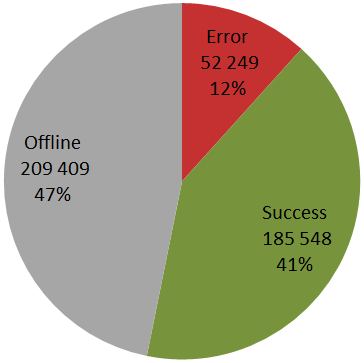
\includegraphics[scale=0.4]{figures/succeed.png}}
    \hspace{10mm}
    \subfigure[Hibák okai]{\label{fig:errors}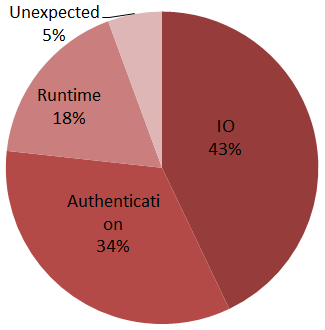
\includegraphics[scale=0.45]{figures/err.png}}
	\caption{Statisztikák\label{fig:statistics}}
\end{center}
\end{figure}

\subsection{Időzített mérési forgatókönyvek}
Az iperf mérések implementálásához új eljárás kidolgozására volt szükség a mérést menedzselő szoftverben. A korábbi traceroute mérések egyetlen parancs távoli futtatásából álltak, amelyek futási eredményét tároltuk el mérési eredményként. Az iperf és más sávszélesség mérő szoftverek működéséhez azonban szükséges mind egy adatcsomagokat küldő és egy adatcsomagokat fogadó példány futtatása a két különböző távoli gépen. Ennek lebonyolításához a mérést lebonyolító programnak több szálon kell futnia, a két távoli kódfuttatást egyszerre kell végeznie. Először az adatcsomagok fogadását (szerver oldal) végző programot kell elindítani, majd csak ezt követően lehet csak a mérést megkezdeni az adatcsomagokat küldő program (kliens oldal) elindításával. A mérést követően a szervert pedig le kell állítani. Ez a szituáció tovább bonyolódik, ha két sávszélesség mérést párhuzamosan szeretnénk végezni. Ez egy fennálló igény, mivel a későbbiekben az MPTCP\footnote{Multipath Transfer Protocol: Több párhuzamos TCP adatfolyamon végez kommunikációt a felsőbb rétegek felé egyetlen TCP kapcsolatot emulálva.} protokoll lehetséges viselkedését is vizsgálni szeretnénk.

Ezeket a lépéseket általánosítva olyan mérési forgatókönyvek létrehozását támogatja már a mérési rendszer, amely bármilyen távoli parancsok időzített futtatását garantálja. Ennek kialakítása a lehető legrugalmasabbra lett tervezve, amelynek működését a függelékben található példakód mutatja be. A kód egyszerűségének ellenére a mérés teljesen menedzselt, bármilyen hiba keletkezése le van kezelve és megfelelően naplózva és a mérési eredményben jelezve van. Garantálva van a helyes időzítés, a párhuzamos futás és a helyes leállás.

%A mérési forgatókönyvek rendkívül hasznosak, segítségükkel új mérések implementálása kényelmes és gyors.